\section{Experiments}
\begin{figure}[t]
	\centering
	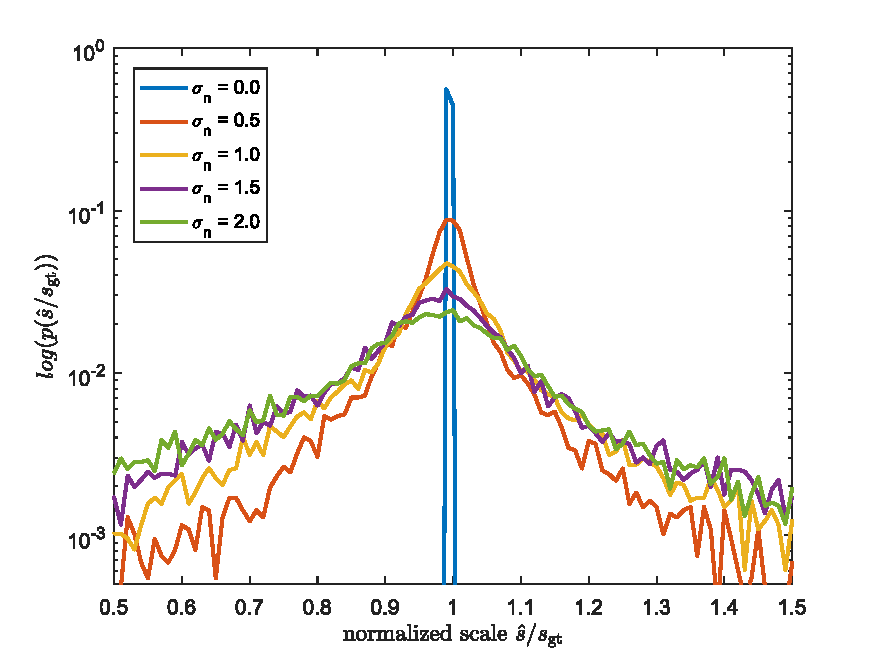
\includegraphics[width=0.5\textwidth]{images/scale_prob_est_e.pdf}
	\caption{}
	\label{experiments:fig:distribution}
\end{figure}
We experiment on a synthetic dataset, with Gaussian-distributed point cloud observed by the pair of pinhole cameras $P_a$ and $P_b$. Both cameras have the resolution 640 by 480 and the focal length 800 pixels. 
Before the cameras are moved, $P_a = \mathrm{I}$. To simulate motion, $P_a$ is moved away from the origin on the surface of a sphere. This generates the cameras as $P_{a'}$ and $P_{b'}$. The direction of motion is random but the distance is neither zero nor far enough to move into the half-sphere opposite to the origin. The principal axis of $P_{a'}$ is ensured to always pass through the center of the sphere. In both cases, $P_b$ maintains a fixed attitude relative to $P_a$. Specifically, it is translated 2 units to the right of $P_a$ on the local x-axis of $P_a$ and rotated 20 degrees around the local z-axis. 

In all tests, both cameras observe a random Gaussian point cloud at the center of the sphere of camera motion. This way there are approximately 100 point correspondences in $P_a$ and $P_{a'}$ and a similar number of correspondences in $P_b$ and $P_{b'}$.

Varying levels of noise between 0 and 2 pixels are added to the points observed in the cameras.  

\subsubsection{Estimate-Distribution Estimate}
Analytically propagating the Gaussian noise through the iterative non-linear essential matrix / relative pose estimator is infeasible. Instead we approximate the distribution through random sampling. We draw $100$ relative pose estimate samples and $\sim 100-500$ second camera correspondences per pose~($\sim 25k$) samples. Specifically we consider the scale estimate quality for each correspondence rather than after 1-pt RANSAC or refinement. 

Figure:~\ref{experiments:fig:distribution} Shows the estimate distribution given varying levels of noise. The figure indicates that the correct answer is the most likely and that any bias is small. This indicates the method should perform well as a initializer for RANSAC-type solvers. 

\subsubsection{Estimate quality given the factor sizes}
\begin{figure}[t]
	\centering
	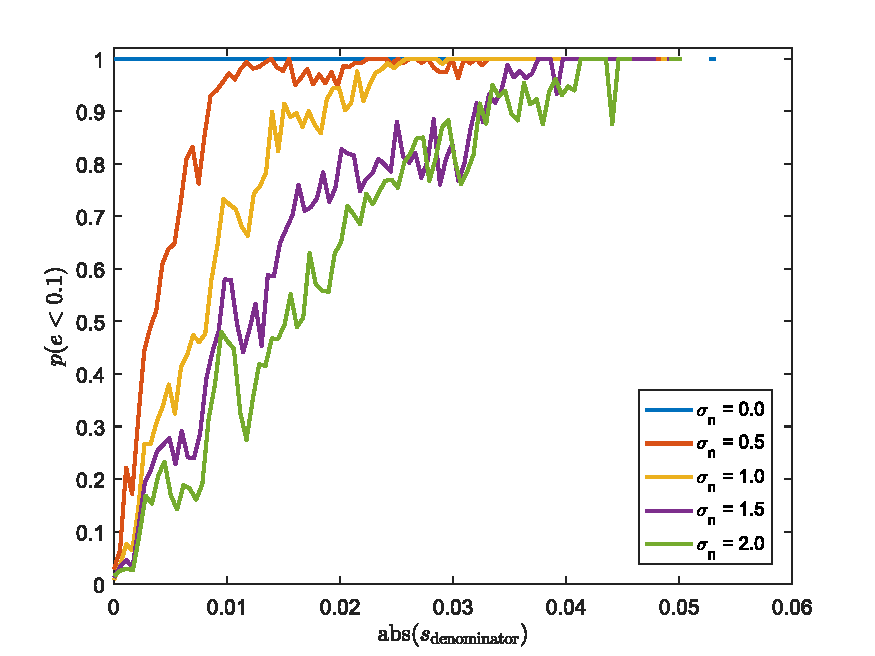
\includegraphics[width=0.5\textwidth]{images/err_prob_denominator_est_e.pdf}
	\caption{}
	\label{experiments:fig:err_prob_denominator}
\end{figure}

\begin{figure}[t]
	\centering
	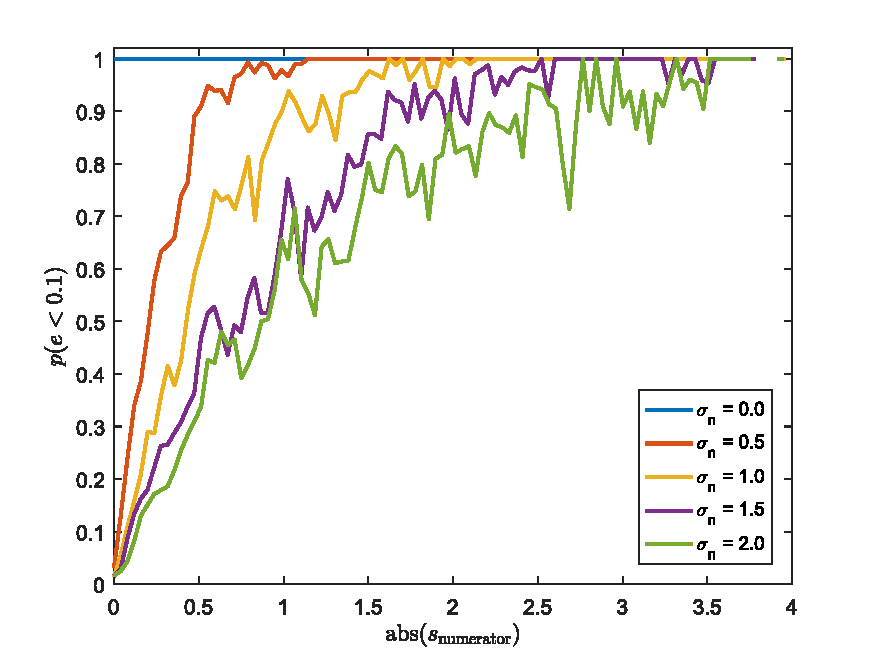
\includegraphics[width=0.5\textwidth]{images/err_prob_numerator_est_e.pdf}
	\caption{}
	\label{experiments:fig:err_prob_numerator}
\end{figure}
Figures~\ref{experiments:fig:err_prob_denominator},~\ref{experiments:fig:err_prob_numerator} validate the hypothesis by showing that with increased values for ($|a|,|b|$) the likelihood of a correct scale estimate is increased and that this effect is stronger with increased noise. The graphs are also sufficient to select a direct threshold based on expected noise statistics. 

